%!TEX root = ../thesis.tex

\chapter{Discussion}
\label{chp:discussion}

In section \ref{sec:ifc-properties}, a set of \gls{ifc} properties based on the work in \cite{Ferraiuolo17} has been introduced; the set of these properties will be referred to as $ P $.
These properties were model checked, the main result of which was a set of rules $ R $ as presented in the previous chapter \ref{chp:results}.
What is the consequence of this?
The formal achievement of this thesis can be summarized as follows:
\begin{quote}
    It can be guaranteed that programs running on the MINRV8 architecture, e.g. \glspl{os}, are \textit{secure} (in the sense of not violating the \gls{ifc} properties $ P $) if they obey to the rules $ R $.
\end{quote}
But what does \enquote{secure} mean here besides not violating $ P $?
What is the \textit{actual} sense of security that can be guaranteed?

At this point, the class of vulnerabilities covered by these properties cannot be defined strictly.
However, the canaries these properties have been tested against in section \ref{sec:canaries}, exemplify this class of vulnerabilities.
Assessing the results of the approach to formally verify higher level properties of the MINRV8 architecture shall be subject of this section.
We will cover five aspects of our work:
\begin{itemize}
    \item Scope, i.e. what are the limits of our results,
    \item trustworthiness, i.e. whether our results are sound,
    \item whether the model could have been implemented more abstractly,
    \item if there are alternatives to tracking information on a per-bit basis, and finally
    \item whether the results meet the self-imposed requirements as set up in chapter \ref{chp:introduction} and section \ref{sec:sum-background}.
\end{itemize}

Whereas the topics of the scope and trustworthiness of our work touch more general aspects of our work, the two questions following up on this reflect on the methodology of this thesis and will elaborate other possible approaches to our subject.

\section{Scope}
\label{sec:scope}

\subsection{Architecture}
\label{sec:discuss-arch}

MINRV8 is meant to be a reasonable abstraction of a real-world RISC-V architecture from a security standpoint.
However, up to this point nothing has been said about the limits of this abstraction.
With every abstraction, there is a small chance that it perfectly matches the concept that has been abstracted in regard to the purpose of the abstraction but in most cases, some corners are cut.
In this section, we will reflect on the limits of the MINRV8 architecture and its implementation.

In summary, the MINRV8 architecture knows three groups of instructions (cf. table \ref{tbl:min-arch-instrs}):
\begin{itemize}
    \item Computational instructions such as \minrv{Mov}, \minrv{And}, \minrv{Add}, etc.
    \item Memory instructions \minrv{Load} and \minrv{Store}
    \item System instructions \minrv{Ecall}, \minrv{Mret}, \minrv{Csrrs}, and \minrv{Csrrc}
\end{itemize}

A reader, experienced in the field of microcontrollers or computer-architecture in general might wonder why our model does not include:
\begin{enumerate}
    \item Executable memory and a \gls{pc}
    \item Jump or branch instructions
\end{enumerate}

The reason for both of these points lies in the implementation of the model.
In the introduction of the MINRV8 architecture in section \ref{sec:minrv8} we mentioned that the idea of the architecture was tightly coupled to its implementation in nuXmv.
The design of the model had to answer the question: How can a stream of instructions be implemented?
nuXmv allows to think of the following options:
\begin{enumerate}
    \item \label{itm:exmem-frozen}
    Use \smv{FROZENVAR}s to model executable memory - a \smv{FROZENVAR} (frozen variable) is something like a constant in other programming languages but without a fixed value.
    nuXmv chooses the value on the first simulation step but does not change it afterwards.
    This is more efficient than using a plain \smv{VAR} and constraining it to not change, e.g. \smv{TRANS next(x) = x;}.
    \item \label{itm:exmem-var}
    Use \smv{VAR}s to model executable memory.
    In practice, this would mean that for memory to hold all instructions executed it would need to be much larger than the current 4 bytes.
    \item \label{itm:exmem-ivar}
    Finally, use \smv{IVAR}s to model the stream of instruction.
    This is the option we decided to go for as described in section \ref{sec:model-implementation}.
    Using input variables means that there is no model of executable memory.
    Instead, the input variables provided to the implementation model a stream of a fully decoded instruction on each transition of the simulated model.
    As such, the architecture does not need to worry \textit{where} these instructions come from.
\end{enumerate}

The decision towards using input variables as a model of the stream of instructions was made because of two reasons:
\begin{enumerate*}[label=\alph*)]
    \item in the prototyping phase of the model, it was quickly found that using input variables led to significant boosts in performance, and
    \item using input variable simplified the implementation significantly.
\end{enumerate*}
Having used purely either frozen variables or variables would have increased the size of the state space to be traversed by nuXmv and would have introduced the necessity to implement instruction decoding increasing the complexity of the transition relation.
Furthermore, it would not have allowed for unbounded model checking of the architecture since the size of programs to be taken into consideration would have been bounded by the size of executable memory.

Yet, using input variables also has some downsides.
First and foremost, using input variables means that it is pointless to model a \gls{pc} or anything address related like return addresses, a dedicated \gls{lr} or \glspl{csr} such as \gls{mtvec}, the \gls{csr} holding the trap-vector base address, as without a model of executable memory there is nothing addresses could point to.
Instead, instructions will simply magically appear on each cycle of the processor model.
This means that the simulation is inaccurate in this regard which in itself is not a problem because the model is supposed to be an abstraction.

\begin{figure}
    \centering
    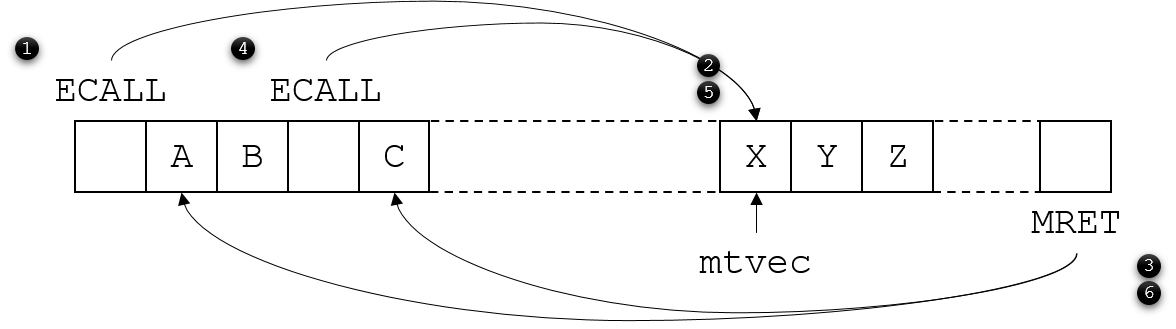
\includegraphics[width=0.7\textwidth]{figures/interrupt-flow.png}
    \caption{Program flow involving interrupts}
    \label{fig:interrupt-flow}
\end{figure}

Since it was decided to use input variables over a model of the \gls{mtvec} register and a \gls{pc}, the question now arises: How accurately is the implementation of the MINRV8 architecture capable of simulating real architectures?

In a nutshell, the use of input variables over (frozen) variables introduces a sense of non-determinism to the model of the MINRV8 architecture when it comes to handling interrupts and exceptions which is illustrated by the following example:
Consider some memory layout for the RISC-V architecture as depicted in figure \ref{fig:interrupt-flow} where code is executed from left to right starting with an \minrv{Ecall} instruction.
Executing this instruction triggers a shift in control to machine-mode which jumps to address \minrv{X} pointed to by the \gls{mtvec} register.
Then, the instructions at addresses \minrv{X} to \minrv{Z} and subsequent ones are executed until finally, a \minrv{Mret} instruction is read an executed which triggers a jump to address \minrv{A}.
Two instructions later, another \minrv{Ecall} instruction is executed, etc.
We would expect the order of instructions to be executed to look something like:

\begin{enumerate}
    \item First environment call: \lstinline[language=minrv8,mathescape=true]{Ecall, Load, Add, Store, $\dots$, Mret}
    \item Return: \lstinline[language=minrv8,mathescape=true]{Load, Mov}
    \item Second environment call: \lstinline[language=minrv8,mathescape=true]{Ecall, Load, Add, Store, $\dots$, Mret}
    \item Second return: \lstinline[language=minrv8,mathescape=true]{Slt, $\dots$}
\end{enumerate}
Where \minrv{Load, Add,} and  \minrv{Store} are the instructions located at addresses \minrv{X} to \minrv{Z} and \minrv{Load, Mov,} and  \minrv{Slt} the instructions located at addresses \minrv{A}, \minrv{B} and \minrv{C} respectively.

However, as input variables cannot be constrained in nuXmv, there is no way to model that the instructions being executed on a trap always are equal, i.e. a valid stream of instructions as a sequence of input variable valuations to the model might be:
\begin{enumerate}
    \item First environment call: \lstinline[language=minrv8,mathescape=true]{Ecall, Load, Add, Store, $\dots$, Mret}
    \item Return: \lstinline[language=minrv8,mathescape=true]{Load, Mov}
    \item Second environment call: \lstinline[language=minrv8,mathescape=true]{Ecall, And, Sra, $\dots$, Mret}
    \item Second return: \lstinline[language=minrv8,mathescape=true]{Slt, $\dots$}
\end{enumerate}

Such a stream of instructions is not realistic without some program modifying the code located at \gls{mtvec} and as such \enquote{should not} be considered when checking the \gls{ifc} properties.
One would expect to find the same code after an \minrv{Ecall} instruction being executed since in both cases, an architecture would jump to the respective interrupt handler\footnote{%
    To be precise, one would also need to take vectored interrupts into account (c.f. sec. \ref{sec:rv-priv-arch}) but even then, the issue applies.
}.
However, there also exists a sequence of input variable valuations that exactly matches a \enquote{real} stream of instructions where the instructions executed after an environment call coincide.

This illustrates one example for why the implementation of the MINRV8 \textit{abstracts} from real architectures.
In regard to program flow on traps, it can be expected that the model accurately comprises all expected streams of instructions but also includes many more one would naturally consider to be unrealistic.

The second concept, the abstract implementation of the MINRV8 architecture is missing are jump an branch instructions.
They are missing for the exact same reasons as described in the previous paragraphs.
Since the implementation does not support executable memory and as such does not support addresses, jumps and branches are pointless instructions.
This, however, does not turn out to be a fundamental problem.

The implementation might not be able to model programs including jumps and branches but the set of programs considered by nuXmv does include traces that include the same instructions that would have been executed when running a program with jumps and branches but without the jumps and branches.
We call such a trace a linearization\footnote{%
    Linearization is similar to function inlining supported by many compilers.
} of a program with jumps and branches.
Consider figure \ref{fig:jump-inlining} where in the upper half depicts an ordinary program, being executed from left to right and including jump instructions.
The respective counterpart to the program in the upper half is depicted in the lower half of figure \ref{fig:jump-inlining}.
This linearized counterpart is considered by nuXmv and the sequence of states generated by the linearized programs is equal to the sequence of states of the non-linearized program modulo \gls{pc} values - which is not modelled in nuXmv anyways.

\begin{figure}
    \centering
    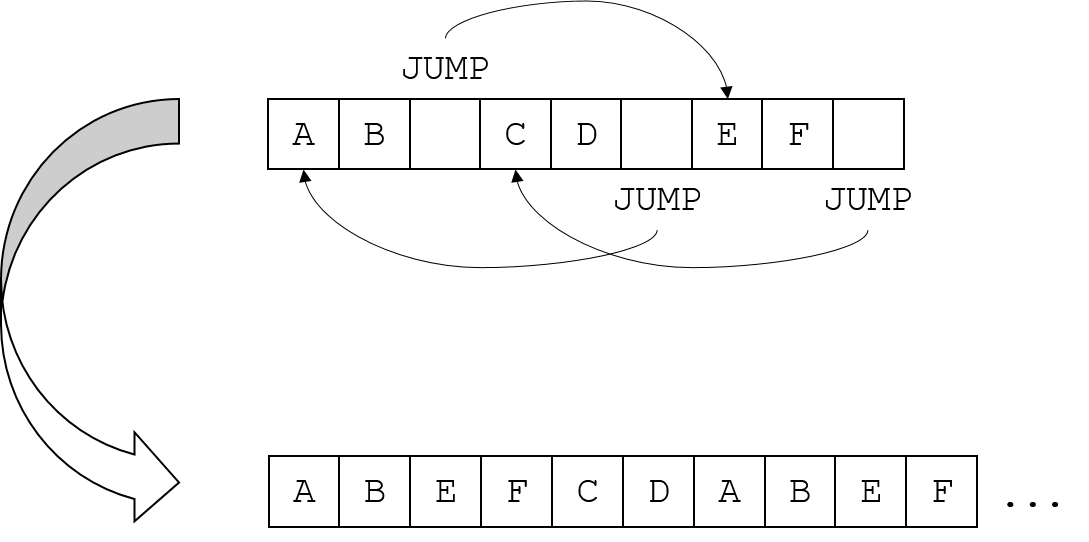
\includegraphics[width=0.7\textwidth]{figures/jump-free-programs.png}
    \caption{Jump linearization}
    \label{fig:jump-inlining}
\end{figure}

\paragraph{Summary}

Starting with the premise of this thesis, it was always clear that the MINRV8 architecture is a simplification.
This, though, is not a problem since by focusing on the very core, security related instructions allowed to implement a tractable and small model in nuXmv.
If one would add jump and branch instructions to the MINRV8 architecture, it'd be fully comparable to actual RISC-V architectures.
From this point of view, it is not a problem to apply the results of the verification process, i.e. the set of assumptions, to the RISC-V architecture.

The implementation of the MINRV8 architecture abstracted from real-world architectures in two main points:
\begin{enumerate}
    \item nuXmv does not guarantee stable behavior on \minrv{Ecall} instructions; this introduces a sense of non-determinism for which there are more programs considered by nuXmv than could actually be run on the MINRV8 architecture.
    This is not problematic because overabstracting the space of all programs $ P $ still leaves nuXmv considering all programs in $ P $.
    \item The implementation does not support jump or branch instructions.
    This is not problematic because programs including jumps can be linearized; such programs \textit{are} considered by nuXmv.
\end{enumerate}

This leaves us with good reasons to assume that programs considered by nuXmv, i.e. the set of programs quantified over when running proofs, is sufficiently close to the set of \enquote{real} programs of the MINRV8 architecture including jumps and branches.

\subsection{Assumptions}

Recall the requirements of the assumptions that have been laid out in section \ref{sec:sum-background}:
\begin{enumerate*}
    \item The assumptions must be non-trivial,
    \item the assumptions must only constrain machine-mode, and
    \item the assumptions must be practical and verifiable.
\end{enumerate*}

In this section, it will be investigated whether the assumptions that ultimately established the correctness of the information flow properties meet all these requirements.

Regarding point \ref{itm:assumptions-non-trivial}, it must be checked that neither are the assumptions contradictory nor do they trivially entail the information flow properties.
Recall that we were able to prove that \enquote{$ \text{assumptions} \Leftrightarrow \text{properties} $}.
In this case, the assumptions could only be contradictory if the properties are as well which they are obviously not as there are valid counter-examples to the properties when no assumptions are given.
On the other hand, recall that in section \ref{sec:canaries} we were able to make changes to the architecture such that \enquote{$ \neg(\text{assumptions} \Rightarrow \text{properties}) $} held.
This indicates that the assumption actually express something meaningful and do not trivially entail the information flow properties.

Point \ref{itm:assumptions-machine-mode} also is met by the assumptions introduced in section \ref{sec:assumptions}.
Whenever it is said that certain instructions must not be executed under certain circumstances, these formulas are guarded by the antecedent \smv{priv ->}.
Additionally, all other assumptions only constrain state transitions being under control of machine-mode only, such as changes to \glspl{csr} or state before machine-mode hands back control to user-mode.

For point \ref{itm:assumptions-verifiable}, meeting point \ref{itm:assumptions-machine-mode} is one step in the right direction.
However, it must remain an open question here whether the assumptions introduced in section \ref{sec:assumptions} can be applied to real-world systems in a verification scenario.
The problems behind this are illustrated by the \smv{SP_BANK} assumption introduced parallel to the SYSRET vulnerability in section \ref{sec:sysret}.
There are two aspects of the first part of this assumption which are noteworthy.
The relevant part of the \smv{SP_BANK} assumption is given in snippet \ref{snpt:sp-bank-p1}.

\begin{figure}
    \begin{lstlisting}[
        language=smv,
        caption={First part of the assumption \lstinline{SP_BANK}},
        label={snpt:sp-bank-p1}
    ]
        G (!priv & X priv -> X ( (*\label{ln:sp-call-priv}*)
            (priv -> !(op in { PUSH, POP }))
            U ((op = MRET & MPP = 0b_0) | sp[sp_sel] < $REGION0_SIZE (*\label{ln:sp-call-mret}*)
                ? !pmpcfg0.write & !pmpcfg0.read
                : !pmpcfg1.write & !pmpcfg1.read)
        )) &
    \end{lstlisting}
\end{figure}

Whilst working on this assumption, it was found that the specific implementation of two \textit{ideas} was critical to the presence of the SYSRET vulnerability, both:
\begin{enumerate}
    \item \label{itm:no-sysret-priv}
    replacing the expression \smv{!priv & X priv} in line \ref{ln:sp-call-priv} by \smv{(op = ECALL) | (bool(MIE) & bool(MEIP))} which is the actual condition under which a trap is taken and
    \item \label{itm:no-sysret-mret}
    omitting the expression \smv{(op = MRET & MPP = 0b_0)} in line \ref{ln:sp-call-mret}
\end{enumerate}
led to nuXmv not reporting the SYSRET vulnerability.
Why is that?

The first part of the \smv{SP_BANK} assumption states: \enquote{Whenever there is a switch from user- to machine-mode, latter can only use the \minrv{Push} or \minrv{Pop} instructions after having returned to user-mode or having ensured that the stack-pointer is safe}.
If the antecedent of this assumption would have been replaced by: \enquote{Whenever a trap is taken, \dots}, i.e. by \smv{(op = ECALL) | (bool(MIE) & bool(MEIP))}, the consequent would also have applied to cases where a trap was taken from machine-mode to machine-mode\footnote{
    Furthermore, it is noteworthy that the antecedent in the original assumption resembles a more result-driven approach to phrasing properties, i.e. talk about \textit{what} is happening, whereas the alternative discussed here resembles a more architecture-driven approach, i.e. talk about \textit{when} things are happening.
    The discussion, which of these approaches should be preferred is a topic on its own.
    In this thesis, we used both approaches but tried to stick to the result-driven approach whenever possible to keep the assumptions concise.
    In certain situations, however, it was more practical to go for the architecture-driven approach.

    A similar issue was discussed by \citeauthor{Reid17} when he elaborates how the properties he verified the ARM architecture against were phrased (cf. \cite[p.88:4]{Reid17}).
}.
Such a trap is critical for the SYSRET vulnerability as it interrupts machine-mode from properly returning to user-mode while already having set the stack-pointer back to user-mode.
The consequent also applying to traps from machine- to machine-mode in context of the MINRV8 architecture leads to machine-mode ensuring that the proper stack-pointer is setup correctly on \textit{all} traps rendering the SYSRET vulnerability impossible.
For example, the \glspl{os} being affected by the SYSRET vulnerability clearly did not set the stack-pointer on \textit{all} execution paths of the trap handler for the general protection fault.

The condition \smv{(op = MRET & MPP = 0b_0)} on the right-hand side of the \smv{U}-expression in line \ref{ln:sp-call-mret} equals telling machine-mode: \enquote{You can forget about not using the \minrv{Push} and \minrv{Pop} instructions after you have \textit{attempted} to return control to user-mode}.
For the same reasons as stated above, this part is critical.
Leaving this expression out would equal machine-mode having state persistent over user-mode-calls and -returns to and from machine-mode, by which machine-mode memorizes whether it has set the stack-pointer to user-mode or to machine-mode.
With such a mechanism in place, machine-mode could not be fooled into using the user-mode stack-pointer on any trap handler since it would first check this state.

These two examples stress that the precise phrasing of the assumptions is critical for both how realistic the assumptions are and how well they might be suited to serve as target for verification of actual code-bases.
While it would be sufficient to find a stronger precondition for these assumptions in existing code-bases, it is non-trivial whether such preconditions are easy to find or whether the assumptions might be rephrased such that they still grant the absence of information flow related bugs but are easier to verify in programs.
This topic, though, cannot be handled as part of this thesis and as such marks future work.

\section{Trustworthiness}
\label{sec:trustworthiness}

Verification processes must not be arbitrary.
The core of verification is to enhance the trust in a given system.
For trust to arise, it is mandatory for the process itself to be trustworthy.

But what does \textit{trustworthy} mean?
\citeauthor{Piano} expressed discussed sense of trustworthiness in his blog post \citetitle{Piano} as:
\textcquote{Piano}{\textins{I}t is extremely difficult to argue convincingly that a verification result is correct. By \enquote{correct} I mean not only \enquote{mathematically sound} but also \enquote{the result is faithful to the intent of the verification effort.}}
Here, we will skip the aspect of technical soundness of this thesis, i.e. the question of whether the work presented in this thesis is without errors.
In consequence, the degree of trustworthiness of this thesis is determined by whether the results of the verification process actually enhance the confidence in the correctness of the MINRV8 architecture, i.e. rather than asking whether what we did was correct, we ask: did we do the \textit{right} thing?

A possible issue with verification is to make circular arguments (an example for this will be given in chapter \ref{chp:related-work}).
Verification engineers do not start their work out of nowhere.
They usually have a feel for what they attempt to verify and have some vulnerabilities in mind they try to tackle.
If the actual work of modeling a prototype and implementing a verification procedure is influenced by this too strongly, one might object:
\enquote{You were able to find vulnerability \textit{X} only because you knew that it was there. Your procedure is nothing but an abstracted simulation of known issues.}

This leads to another concern:
As with most programming, the verification process will tackle what is aimed for in some more general sense, i.e. when aiming to verify systems against certain bugs these are usually generalized to classes of related vulnerabilities.
But with such an approach, one can never be sure that there is no other class of vulnerabilities that was missed.
In other words: Does the verification procedure have blind spots?

It will now be investigated whether this work is touched by aforementioned two issues.

First, it will be investigated whether a circular argument has been made in this thesis.
Recall the steps that have been taken to verify the MINRV8 architecture against the information flow properties:
\begin{enumerate}
    \item \label{itm:step-minrv}
    Specify the MINRV8 architecture based on RISC-V
    \item \label{itm:step-semantics}
    Define information flow semantics for the instructions available on MINRV8
    \item \label{itm:step-properties}
    Use fields not being propagated in the information flow semantics and some intuition to state information flow properties
    \item \label{itm:step-loop}
    Enter a prove-refine loop until a fixpoint has been reached
    \item \label{itm:step-canaries}
    Test the model by subjecting it to vulnerabilities
\end{enumerate}

We find that steps \ref{itm:step-semantics} to \ref{itm:step-loop} are well founded by both theory and intuition and do obviously not face the risk of making a circular argument.
This, however, is less obvious for steps \ref{itm:step-minrv} and \ref{itm:step-canaries}.
In both cases, the selection of RISC-V features and instruction to include or vulnerabilities to test respectively can be doubted.

The work on this thesis was indeed influenced by the canaries the model was ultimately tested against, e.g. it was decided to implement a cache to be able to cover the cache poisoning attack, and vice versa: the selection of vulnerabilities to test the model against was based on the features implemented in it.
Despite the circular character of these two steps, we find that this is not an issue.
Steps \ref{itm:step-minrv} and \ref{itm:step-canaries} must be understood as a prototype of a verification procedure proposed in this thesis which is given by steps \ref{itm:step-semantics} to \ref{itm:step-loop}.
Having the setup to test these steps being derived via a methodology that is circular to some degree does not make the procedure itself circular.
The opposite is the case:
We find that the definition of information flow semantic, information flow properties and the prove-refine loop are all well founded and comprehensible, i.e. follow intuition.
On the other hand, we must admit that it is unknown whether there are blind spots to the verification procedure or more precisely: to the information flow properties.

We argue that our results are indeed trustworthy as we managed to show that our properties are not meaningless since they are able to detect both the SYSRET and the cache poisoning vulnerability and well founded in intuition.
But it is unclear
\begin{enumerate*}[label=\alph*)]
    \item which class of bugs or vulnerabilities can be detected by this procedure and
    \item whether this class covers \textit{all} vulnerabilities in the sense of \citeauthor{Piano}, i.e. \textcquote{Piano}{the result is faithful to the intent of the verification effort.}
\end{enumerate*}
We mark this problem as future work.

\section{Abstract Model}

One might ask, why it was decided to simulate all flows of information through the model of the MINRV8 architecture and indeed: In scope of this thesis, the actual content of registers is not mandatory, i.e. the actual contents of registers could be removed from the model such that only information flow tracking labels are tracked.
Register values do play a role when memory is indexed, but this could likely be abstracted by non-deterministically choosing a memory location to be targeted by loads and stores.

There are two reasons for why this decision was made.
Firstly, since the work of \citeauthor{Ferraiuolo17} \cite{Ferraiuolo17} was adopted where the authors did rely on precise values to track\footnote{%
    This is due to the fact that \gls{hdl} code is annotated.
    Or in other words: the authors did not have a chance to not track precise values.
} and performance of nuXmv did not mandate to shrink the model, it initially was decided to model values in the MINRV8 architecture.

However, secondly, working with concrete values has two benefits which might become important in future work.
\begin{enumerate}
    \item If the model ever was to be extended by jumps and branches, deterministic addresses are needed to model static code in executable memory.
    If not only loads and stores but also jumps and branches would use non-deterministic mechanisms to determine target addresses, modelling executable memory (cf. sec. \ref{sec:discuss-arch}) and for example interrupt handlers located in this very memory would be pointless to begin with.
    \item Concrete values lead to counter-examples being easier to interpret.
\end{enumerate}

With these two reasons at hand and the overall goal of this thesis to implement a prototype for a methodology to verify \glspl{isa}, we find that having modelled register values as opposed to abstractly tracking information flow labels only improves on the significance of our results.

\section{Per-Bit Information Flow Tracking}
\label{sec:per-bit-tracking}

Another issue is that in chapter \ref{chp:results} it was mentioned that counter-examples never involved flows of information where the bit-wise labels of values in the architecture was critical.
In other words: for this thesis, tracking only one bit for confidentiality and one bit for integrity for each register and memory address would suffice.
Initially, it was decided to track labels bit-wise because \begin{enumerate*}[label=\alph*)]
    \item we followed the approach of \citeauthor{Ferraiuolo17} \cite{Ferraiuolo17} which tracked information flow bit-wise as well,
    \item again, performance was sufficient to allow for it, and
    \item one couldn't have been sure prima facie non-bit-wise tracking of information would suffice.
\end{enumerate*}

Additionally, it can also be seen that computational instructions never played a major role in any counter-example.
These results suggest that in future work, if the model ever was to be expanded to a more accurate model of RISC-V and/or to a higher machine-word width and performance problems then are encountered, one could abstract the information flow tracking labels from bit- to word-wise labels.
This would decrease the size of the state space to be considered by nuXmv exponentially.
Additionally, one could remove instructions that only alter data but do not add \enquote{new} ways for information to flow.
E.g. the \minrv{Add} instruction - from a pure standpoint of \textit{where} information flows - adds nothing in comparison to the \minrv{Mov} instruction.
This option only shrinks the state space by a linear factor - nevertheless it might matter.

The gist of these findings is:
Whereas in the work of \citeauthor{Ferraiuolo17} \cite{Ferraiuolo17} tracking of each and every bit for a given system was crucial because the authors \textit{could not choose where bugs occur}, it seems that in our more-high level approach, for every bug \enquote{imaginable}, there is a very simple trace illustrating it: nuXmv is able to choose where a bug occurs since it quantifies over programs as opposed to the work of \citeauthor{Ferraiuolo17} where the program of interest is fixed.

\section{Requirements}
\label{sec:discuss-requirements}

In the introduction, three goals were set for this thesis: it was claimed that the approach presented as part of this thesis is \textit{viable}, i.e. feasible, realistic and generalizable, \textit{effective}, i.e. it is able to detect issues, and \textit{supplemental}, i.e. it enhances on related work.

All proofs were run on a laptop equipped with an Intel Core i7-7500U CPU and 8GB of RAM.
It is safe to say, that these are very moderate hardware requirements.
Proofs were conducted per property.
None of these proofs took more than 60s.
While we can give no clear count of working hours spent on this thesis, all of it was developed and written by a single person in no more than nine months.
During this time, this person did not solely work on this thesis.
In a non-research scenario one can assume that development would be more straight forward since it would not include the definition of an architecture.
Due to the exponential blow-up of binary encoded state spaces, there are no guarantees that this approach scales well to realistic and complete architectures.
However, there are two reasons which make seem likely that this approach does indeed scale.
Firstly, the proofs here were ran on a small machine and did not take much time.
Secondly, in sections \ref{sec:per-bit-tracking} it was discussed that bit-wise tracking of information flow might be dropped, i.e. there is room for performance improvements.
All of this gives good reasons to believe that our approach is indeed \textit{viable} and could be applied to other architectures with reasonable effort.

To discuss the \textit{relevance} of this work, recall that in section \ref{sec:assumptions} it was shown that the implementation of the MINRV8 architecture models the property \enquote{assumptions $ \Leftrightarrow $ properties}.
This was put to a test by exposing the implementation to the cache poisoning or SYSRET vulnerability where it was found that it then does violate the properties as presented in section \ref{sec:ifc-properties}.
In other words: it was shown that the three properties \smv{MEMORY_OP_INTEGRITY}, \smv{CSR_INTEGRITY} and \smv{NO_LEAK} cover at least vulnerabilities related to the cache poisoning or SYSRET vulnerability without any manual intervention besides changing the architecture itself.
This marks the main result of this thesis and shows that our approach to verifying \glspl{isa} is \textit{effecitve}.
Furthermore, mitigations to these vulnerabilities can be verified using the same model.
It must be decided on a case by case basis whether a given violation of the information flow properties actually marks a vulnerability of the architecture leaving it with the need to be altered or marks a feature the risks of which must be controlled in software.

The discussion whether our work also is \textit{supplemental} will be postponed to a later stage.
In the following chapter \ref{chp:related-work}, related work will be presented.
Following up on this, this discussion will be picked up.

In addition to these self-imposed goals, it was also decided in section \ref{sec:verify-spec} to adopt the four design goals that were initially introduced in \cite{Reid17}.
These were defined to apply to high level properties for specifications and list as follows:
\begin{displaycquote}[pp.88:2-3]{Reid17}
    The central design challenge we face is to create a set of properties that:
    \begin{itemize}
        \item express the major guarantees that programmers depend on;
        \item are concise so that architects can easily review and remember the entire set of properties;
        \item are stable so that architectural extensions do not invalidate large numbers of rules;
        \item and that describe the architecture differently from existing specification to reduce the risk of common-mode failure.
    \end{itemize}
\end{displaycquote}

These objectives are met by our work:
\begin{itemize}
    \item The assumptions give rules for programmers of \glspl{os} and compilers that guarantee programs adhering to these do not violate basic information flow properties.
    \item Both assumptions and properties are small in number and short and can be expressed in intuitive natural language, hence are concise.
    \item The properties itself are completely architecture independent and as such stable.
    The assumptions are architecture dependent and rely on both instructions available and concrete semantics of these instructions.
    However, we feel subjectively that only basic mechanics are used and predict that the assumptions in a practical environment of an architecture should be relatively stable as well.
    \item The premise of information flow tracking on instruction level is to describe the architecture from a different point of view.
    It is therefore obvious that there is very little risk of common-mode failure.
\end{itemize}
